\documentclass{standalone}

\begin{document}

\subsection[mRNA data]{mRNA dataset}\label{synapse:mRNA}

We applied both training procedure (ref. Fig.~\ref{fig:dnet_pipe}) on the mRNA dataset.
The results are shown, as distribution of AUC (Area under the curve) score, in Fig.~\ref{fig:dnet_results}~(a) for the best signatures obtained with procedure $A$ (corresponding to the validation approach used in~\cite{Yuan2014}), while results with the full cross-validation procedure $B$ are shown in Fig.~\ref{fig:dnet_results}~(b).

As expected, performances decrease with the introduction of the second cross validation step, but the values remain quite stable showing the robustness of the extracted signatures, and we remark that the validation procedure used in the reference paper by Yuan et al. resembles our approach without the second validation step.

\begin{figure}[htbp]
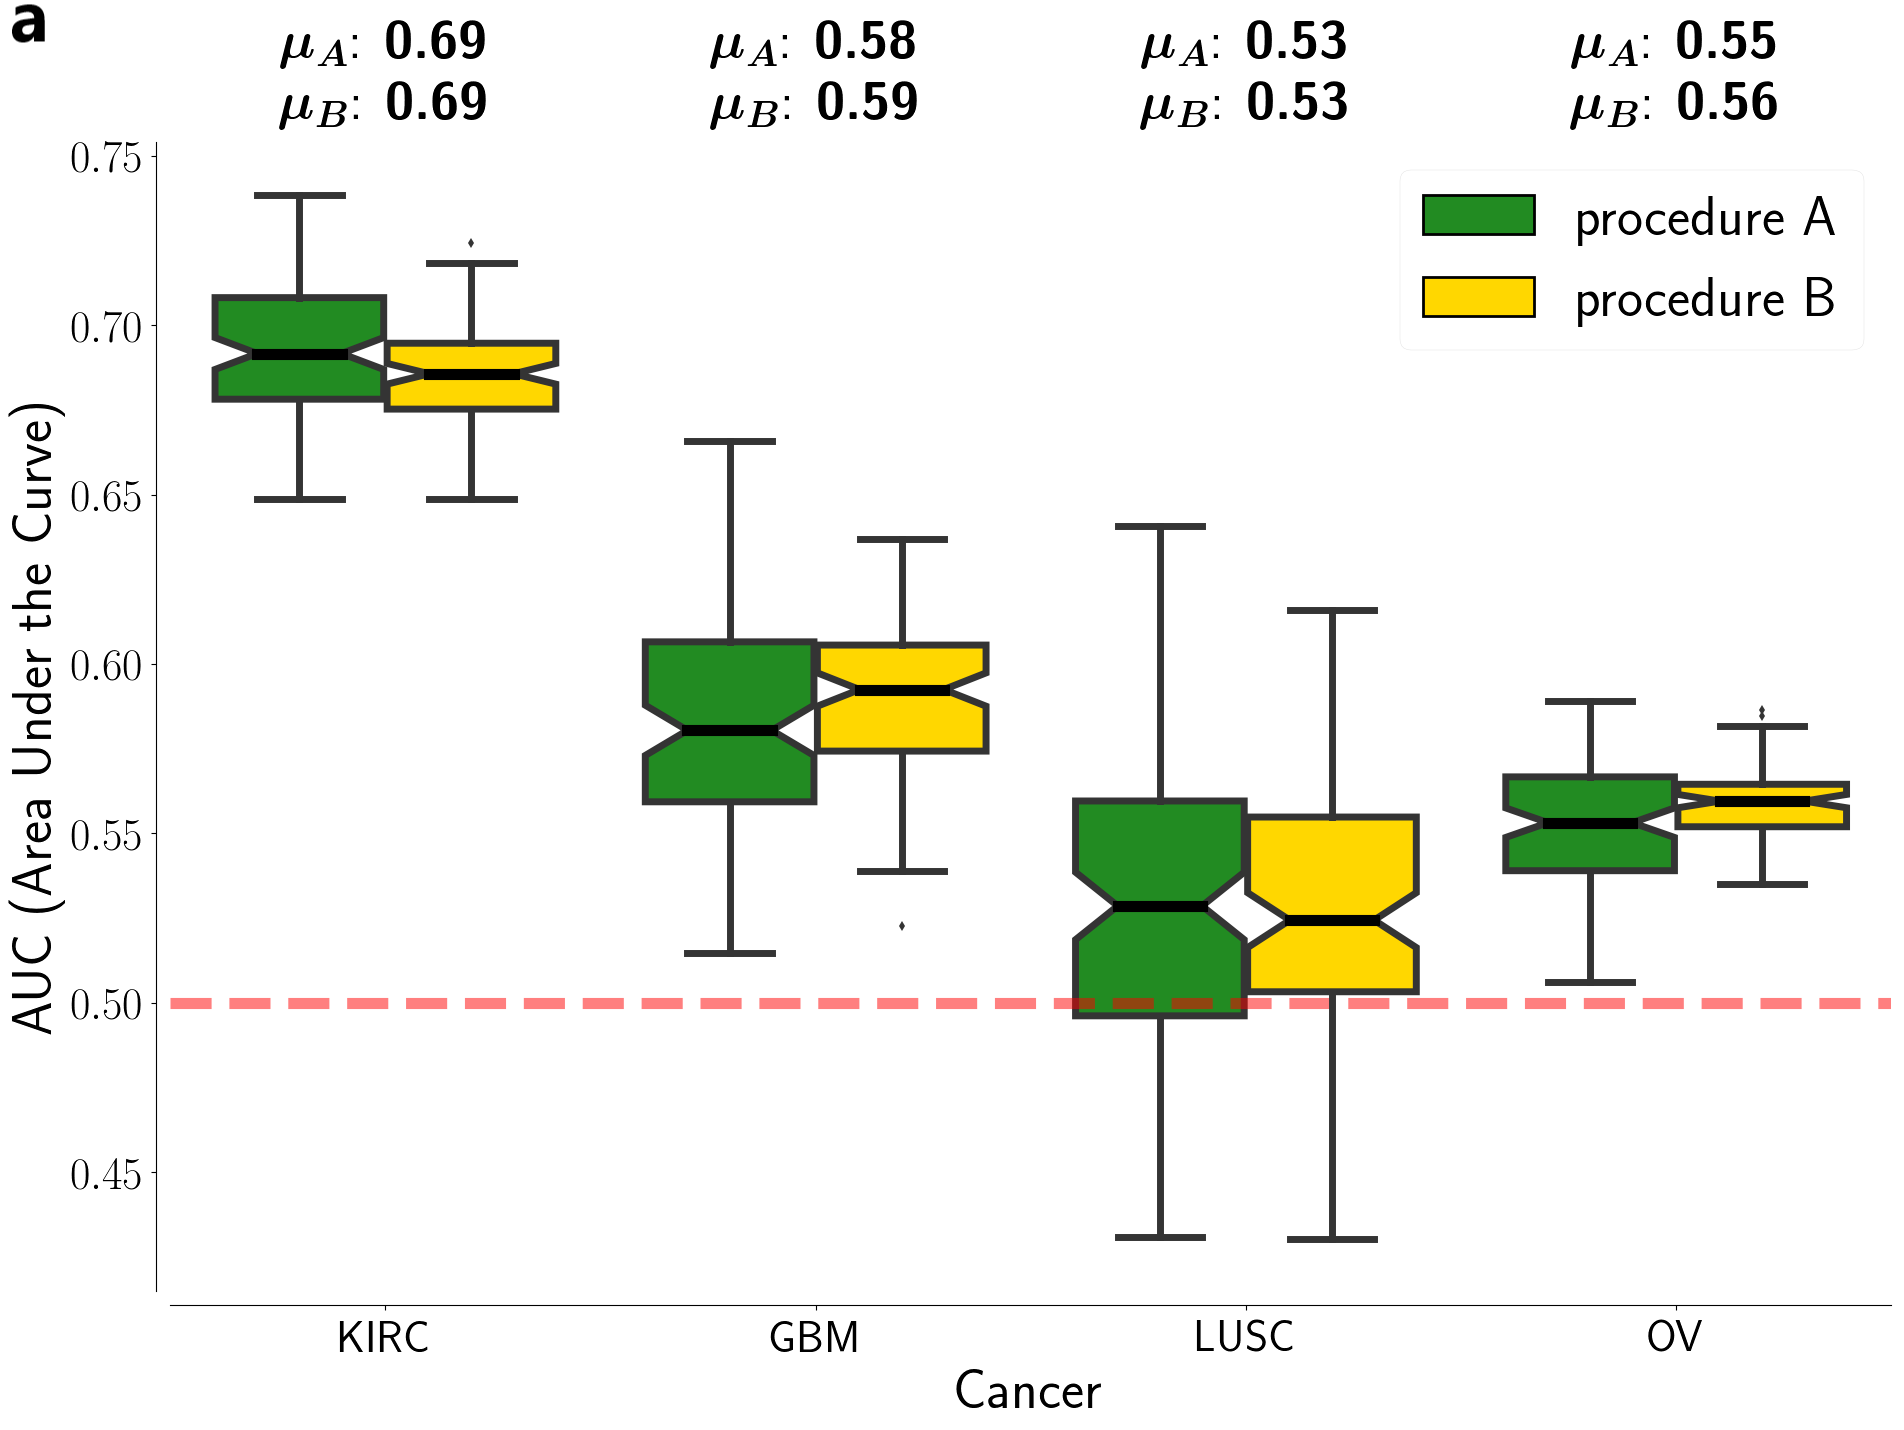
\includegraphics[width=0.4\textwidth]{mRNA_boxplot.png}
\qquad
\centering
\def\svgwidth{0.45\textwidth}
\input{./img/mRNA_tables.pdf_tex}
\caption{Results obtained by the \textsf{DNetPRO} algorithm pipeline on four mRNA tumor datasets, as from the Synapse database~\cite{Yuan2014}.
\textbf{(a)} Distributions of AUC values for the tumor datasets. Green boxplots: results using procedure $A$ as described in Fig.~\ref{fig:dnet_pipe}; yellow boxplots: results obtained using procedure $B$.
\textbf{(b)} Comparison of \textsf{DNetPRO} results with the methods used in the paper of Yuan et al.: max AUC values obtained over the 10-Fold cross-validation procedure.
}
\label{fig:dnet_results}
\end{figure}

All results are comparable (LUSC) or better (KIRC, GBM) than the results reported in~\cite{Yuan2014}, except for the OV dataset, also with the more conservative approach involving a further cross-validation step.
The size of the extracted signatures is quite constant, and smaller than 500 genes in each pipeline execution.

To test the robustness of our method, since each cross-validation procedure may generate different signatures, we measured the overlap of the genes belonging to each mRNA signature over 100 simulations with different training-test data splitting.
We observed an average overlap ranging from 40\% to 60\%, with a smaller group of genes found across all the 100 cross-validation iterations.

In this application the \textsf{DNetPRO} algorithm has several advantages: easy scalability on parallel architectures, simple signature interpretation allowing a valuable application in a biomedical context and a significant robustness in a highly noisy environment such as genomics measurements.

\end{document}
